The given PDF graph can be represented by the function $f(x)$.
\begin{align}f(x)=
\begin{cases}
0 & |x|>1
\\ 1-|x| &|x|\le 1
\end{cases}
\end{align}
The CDF can be expressed as 
%Now,we need to find the corresponding CDF graph for f(x).let the CDF represented by F(x).we know that

\begin{align}
    F(x)&=\int_{-\infty}^{x}f(x)dx 
    &=
    \begin{cases}
 \int_{-1}^{x}(1+x)dx & x\in[-1,0)
\\
\int_{0}^{x}(1-x)dx & x\in(0,1]
    \end{cases}
\end{align}
% or, 
\begin{align}
    F(x)=
\begin{cases}
0 &|x|>1
\\ \frac{x^2}{2}+x+\frac{1}{2} &-1\leq x <0
\\ \frac{-x^2}{2}+x+\frac{1}{2} &0\leq x <1
\end{cases}
\end{align}
and plotted in  Fig. \ref{var/1/fig:CDF graph}.
\begin{figure}
\centering
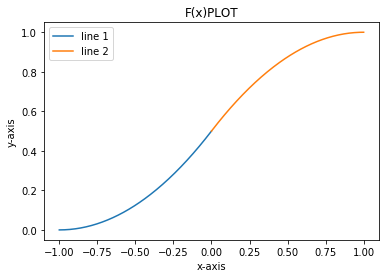
\includegraphics[width=\columnwidth]{variable/solutions/1/graph.jpg}
\caption{CDF graph}
\label{var/1/fig:CDF graph}
\end{figure}






